\begin{tikzpicture}[transform shape]
    % Define coordinates for the main elements
    \coordinate (leftImg) at (0,0);
    \coordinate (topImg) at (5,2.5);
    \coordinate (bottomImg) at (5,-2.5);
    \coordinate (rightEq) at (10,1.0);
    
    % Place the placeholder images (blue rectangles with numerical solution)
    \node[inner sep=0] (leftRectangle) at (leftImg) 
        {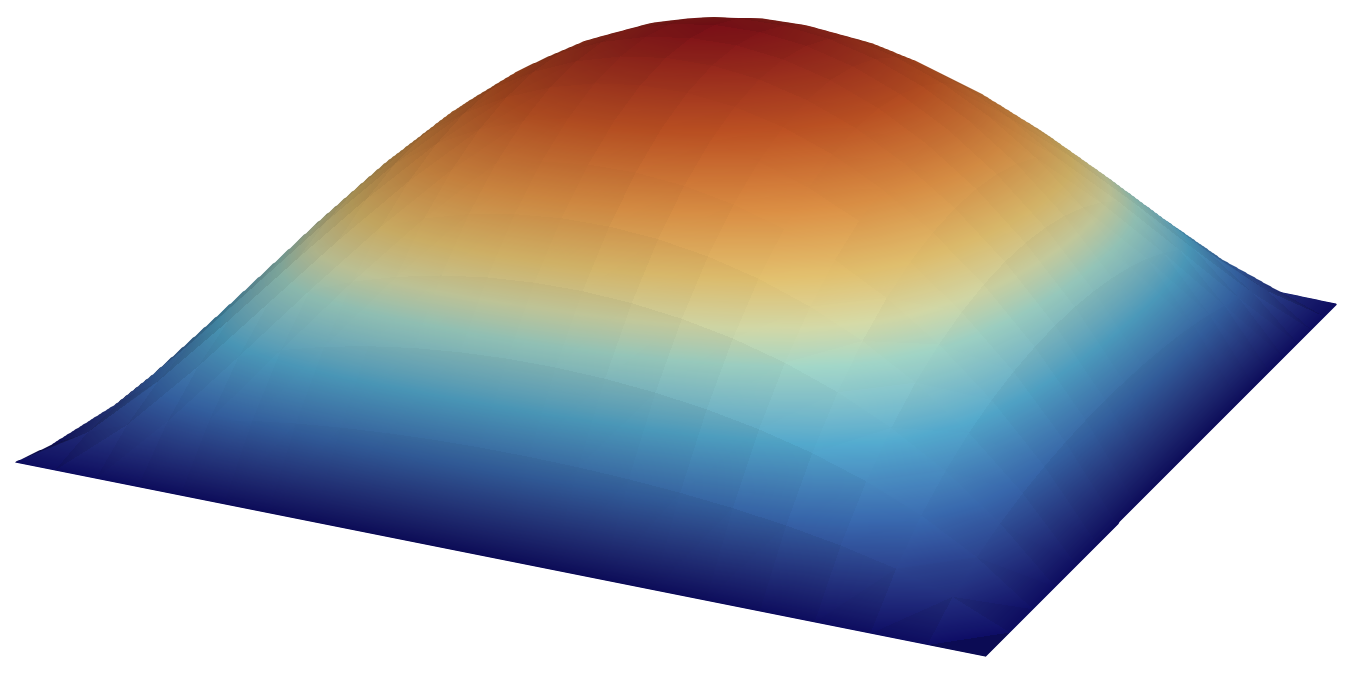
\includegraphics[width=5cm]{images/global-solution.png}};
    \node[inner sep=0] (topRectangle) at (topImg) 
        {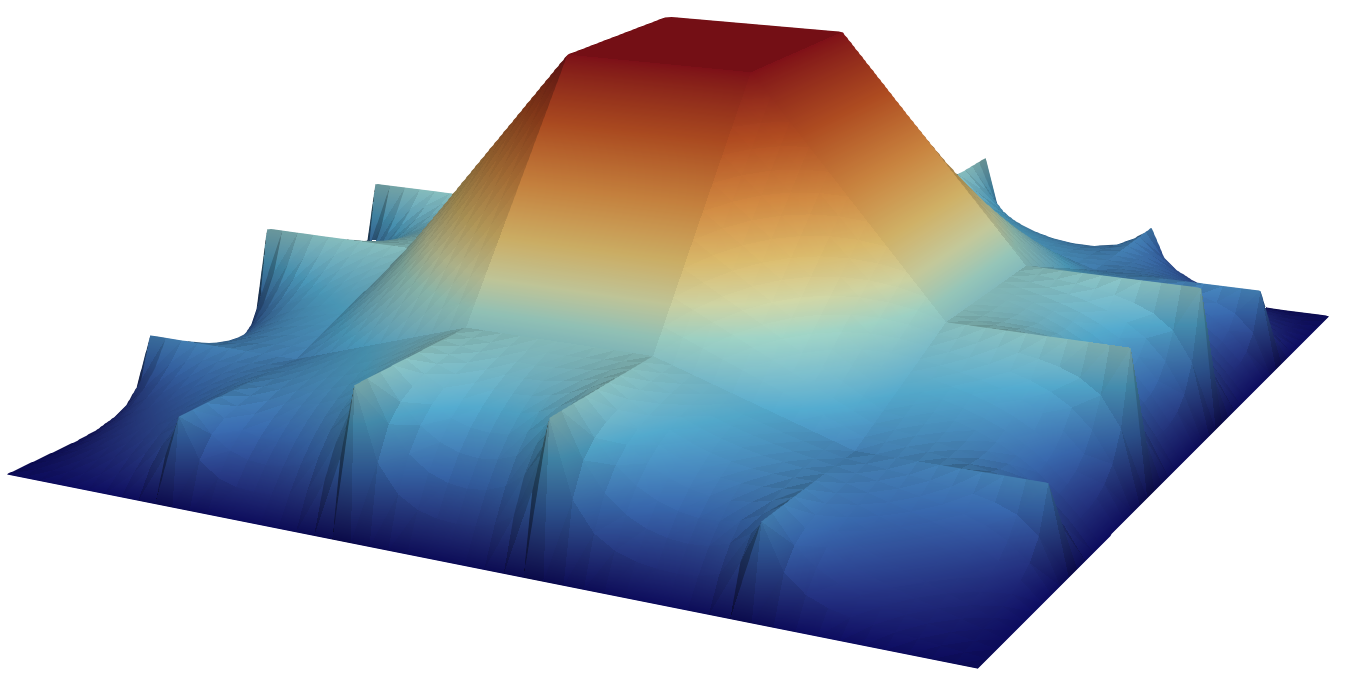
\includegraphics[width=5cm]{images/coarse-solution.png}};
     \node[inner sep=0] (bottomRectangle) at (bottomImg) 
        {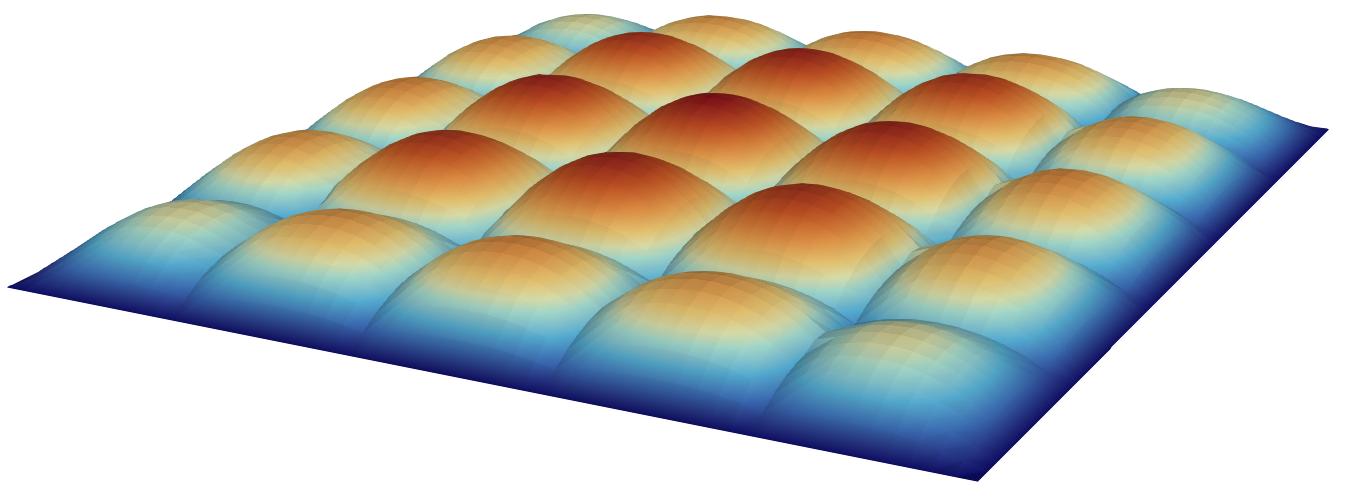
\includegraphics[width=5cm]{images/local-solutions.png}};
    
    \node[fill=white, fill opacity=0.7, text opacity=1, yshift=5mm, xshift=2mm, text width = 35mm] at (leftRectangle.north) {\small Discretized nonlinear problem};
    \node[yshift=0cm, fill=white, fill opacity=0.9, text opacity=1] at (leftRectangle.south) {\small $F(u) = 0$};

    \node[yshift=0cm, fill=white, fill opacity=0.9, text opacity=1] at (bottomRectangle.south) {\small $R_i F\left(\bm{u} - R_i^T T_i(\bm{u})\right) = 0$};
    
    \node [fill=white, fill opacity=0.9, text opacity=1] at (topRectangle.south){\small $\Phi^T F\left(\bm{u} - \Phi T_0(\bm{u})\right) = 0$};
    
    \node[align=left, fill=white, fill opacity=0.7, text opacity=1, text width = 4.5cm] at (9.6,-1.3){\small Solve with Newton's method for nonlinear corrections $T_i(u), \quad i = 0,\ldots, N$};
    
    \node[draw, rectangle, minimum width=4cm, minimum height=1cm] (boxedEq) at (rightEq) {\small $\mathcal{F}(\bm{u}) = \sum_{i=0}^{N} R_i^T T_i(\bm{u})$};
    
    % Arrows
    \draw[-{Stealth[length=3mm, width=2mm]}] ($(leftRectangle.north east) + (-0.5, -0.5)$) -- ($(topRectangle.south west) + (0.3, 0.3)$);
    \draw[-{Stealth[length=3mm, width=2mm]}] ($(leftRectangle.south east) + (-0.7, 0.4)$) -- ($(bottomRectangle.north west) + (0.8, -0.2)$);
    \draw[-{Stealth[length=3mm, width=2mm]}] ($(topRectangle.south east)+ (-0.3, 0.7)$) -- ($(boxedEq.north west)+ (-0.1, 0.1)$);
    \draw[-{Stealth[length=3mm, width=2mm]}] ($(bottomRectangle.north east)+ (-0.8, -0.1)$) -- ($(boxedEq.south west)+ (-0.1, -0.1)$);
\end{tikzpicture}
